% !TeX program = xelatex
\documentclass[UTF8]{ctexart}

\usepackage{amsmath, amssymb}
\usepackage{booktabs}
\usepackage{graphicx}
\usepackage{float}
\usepackage{geometry}
\usepackage{hyperref}
\usepackage{url}

\geometry{a4paper, margin=2.5cm}
\pagestyle{plain}
\ctexset{
  section = {
    format = \Large\bfseries\raggedright
  }
}
\hypersetup{
  colorlinks=true,
  linkcolor=blue,
  citecolor=blue,
  urlcolor=blue
}
\renewenvironment{abstract}
  {\begin{center}
   {\large 摘要\par}
   \vspace{0.5em}
   \begin{minipage}{0.92\linewidth}
   \normalfont\normalsize}
  {\end{minipage}
   \end{center}}

\title{大语言模型能改变金融投诉的表达方式吗？来自 CFPB 消费者投诉数据的文本分析证据}
\author{周奕博}
\date{}

\begin{document}

\maketitle
\begingroup
\renewcommand{\thefootnote}{}
\footnotetext{数据集来自美国消费者金融保护局（Consumer Financial Protection Bureau, CFPB）公开的 \href{https://www.consumerfinance.gov/data-research/consumer-complaints/}{Consumer Complaint Database}。代码、实验数据和复现方式已上传至 \href{https://github.com/zhoudapig13/big-data-analysis-course-paper-data}{GitHub 仓库：大数据分析课程论文数据}。}
\endgroup

\begin{abstract}
大语言模型正在改变个人撰写正式文本和与机构沟通的方式，但这种变化是否已经进入金融消费者投诉场景，仍缺乏基于大规模真实文本的经验证据。本文使用 CFPB Consumer Complaint Database 中 2015--2026 年的 30,263 条消费者金融投诉，考察 ChatGPT 发布前后投诉文本表达、投诉主题结构和企业响应结果的变化。本文构建一个结合文本特征、主题建模和可解释机器学习的分析框架：首先从投诉叙事中提取法律化表达、证据组织、模板化短语、词汇多样性和文本长度等表达变量；其次基于相似历史投诉构造局部表达变化得分，以控制产品、公司、地区和争议事项差异；最后将文本表示、主题标签和结构化变量输入响应预测模型，并使用特征解释方法分析表达信号与及时回应、金钱救济和非金钱救济之间的关系。初步结果显示，后 ChatGPT 时期投诉文本的法律术语和模板化表达明显增加，同时企业非金钱救济比例和整体救济响应率也出现上升趋势。这些发现提示，LLM 可能正在通过重塑消费者的正式表达方式影响金融纠纷中的信息呈现和机构响应过程。本文不将这种相关性直接解释为因果效应，而是提供一个可复现的文本分析框架，为研究生成式 AI、消费者保护和平台化监管之间的关系提供经验基础。

\noindent\mbox{关键词：大语言模型；金融消费者投诉；CFPB；文本分析；可解释机器学习；企业响应}
\end{abstract}

\section{引言}

大语言模型（Large Language Models, LLMs）正在改变个人与机构沟通的方式。与搜索引擎或传统文本模板不同，LLM 不仅能够提供信息检索，还能够帮助用户组织事实、补充法律化表达、调整语气并生成较为完整的正式文本。因此，在金融消费者投诉这一高度依赖书面表达的场景中，LLM 可能不仅是一个写作辅助工具，也可能成为影响消费者表达能力、投诉可读性与企业响应结果的重要技术变量。

金融消费者投诉是观察这一变化的理想场景。一方面，消费者在面对银行、信用卡公司、征信机构、贷款服务商和债务催收机构时，往往处于信息和专业知识相对弱势的位置；另一方面，投诉文本又需要在有限篇幅内同时呈现事实经过、权利主张、证据线索和救济请求。美国消费者金融保护局（Consumer Financial Protection Bureau, CFPB）建立的 Consumer Complaint Database 收集了消费者关于金融产品和服务的投诉，并记录产品类型、争议事项、投诉叙事、企业回应和是否及时回应等字段，为研究金融市场中的消费者表达与企业响应提供了大规模公开数据基础\cite{cfpb_database,cfpb_fields}。

已有研究表明，消费者投诉文本并非简单的非结构化材料，而是可以通过机器学习方法提取风险主题、市场趋势和制度信号。Bastani 等人利用 LDA 主题模型分析 CFPB 投诉叙事，展示了主题建模在识别金融投诉潜在议题和时间趋势方面的价值\cite{bastani2019lda}。随着预训练语言模型和神经主题模型的发展，文本分析不再局限于词频统计，而可以进一步刻画语义结构、叙事模式和表达风格\cite{grootendorst2022bertopic}。这些方法为本文提供了一个基本出发点：金融投诉不仅可以被视为事件记录，也可以被视为一种具有策略性和制度嵌入性的文本表达。

然而，LLM 的出现使这一问题变得更加复杂。近期关于 CFPB 投诉的研究发现，ChatGPT 发布后消费者投诉中可能出现了 LLM 辅助写作的迹象，并进一步讨论了 LLM 使用与获得企业救济之间的关系\cite{shin2026llmcomplaints}。与此同时，DetectGPT 等机器生成文本检测方法说明，LLM 生成文本可能在概率结构和语言分布上呈现不同于人类文本的特征\cite{mitchell2023detectgpt}。这些研究提示我们：如果消费者借助 LLM 起草投诉，投诉文本可能在长度、句式、法律术语、证据组织、情绪表达和模板化程度上发生变化；而这些变化又可能影响企业对投诉的理解、分类和回应。

本文关注的问题是：LLM 能否改变金融投诉的表达方式？更具体地说，本文试图回答三个相互关联的问题。第一，后 ChatGPT 时期的金融投诉文本是否呈现出更强的法律化、模板化或结构化表达特征？第二，不同风险主题和产品类别下，投诉表达变化是否存在异质性？第三，这些文本表达特征是否与企业是否提供金钱救济、非金钱救济或及时回应存在系统关联？与仅仅判断投诉是否由 AI 生成不同，本文更关心 LLM 作为一种表达增强技术，是否改变了消费者在金融纠纷中的叙事方式和可见性。

\begin{figure}[t]
  \centering
  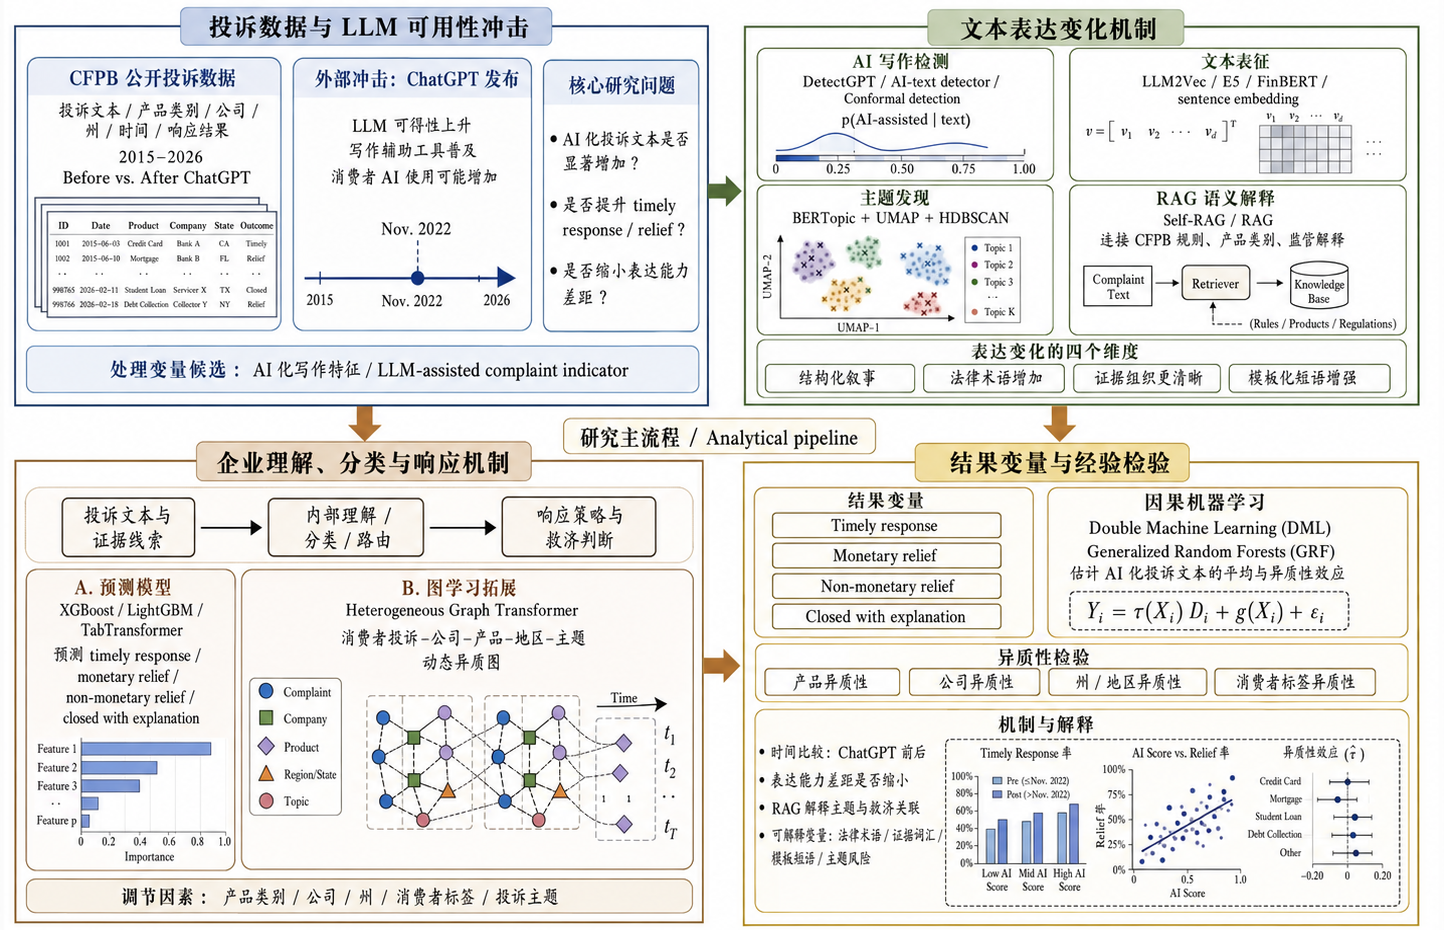
\includegraphics[width=\linewidth]{figures/fig1_llm_complaint_framework_cropped.png}
  \vspace{1em}
  \refstepcounter{figure}
  \label{fig:mechanism-framework}
  \begin{minipage}{0.96\linewidth}
    \raggedright
    \small
    \textbf{Figure~\thefigure.} LLM 辅助金融投诉文本转变、企业响应与经验检验框架。图中展示了 CFPB 投诉数据、ChatGPT 发布后的 LLM 可用性冲击、文本表达变化检测、企业理解与响应机制，以及结果变量和因果机器学习检验之间的关系。底部模块进一步概括了产品类别、公司、地区、消费者标签和投诉主题等调节因素。
  \end{minipage}
\end{figure}

为回答上述问题，本文基于 CFPB 消费者投诉数据构建一个文本分析与可解释机器学习框架。首先，本文对投诉叙事进行清洗和标准化处理，并构造文本长度、句长、词汇多样性、法律术语、证据词、紧迫性词语、困难处境词语和模板化短语等表达特征。其次，本文使用主题建模识别投诉中的主要风险议题，并比较不同主题下的表达方式与企业响应差异。最后，本文以企业救济响应和及时回应为结果变量，建立可解释预测模型，分析哪些文本信号与企业响应结果相关。该框架并不将相关性直接解释为因果效应，而是将其作为进一步机制分析和稳健性检验的基础。

本文的潜在贡献体现在三个方面。第一，在研究对象上，本文将 LLM 时代的文本表达变化引入金融消费者保护场景，补充了以往侧重投诉主题识别或企业响应结果预测的研究。第二，在方法上，本文将文本统计特征、主题模型和可解释机器学习结合起来，使金融投诉文本既可以被描述为风险主题分布，也可以被解释为影响响应机制的表达信号。第三，在社会科学意义上，本文讨论 LLM 是否可能降低消费者表达门槛、增强弱势消费者的正式沟通能力，同时也提醒我们注意模板化投诉、检测偏误和企业响应自动化带来的新挑战。

总之，本文并不把 LLM 视为一个单纯的技术工具，而是将其放入金融消费者、企业和监管平台之间的互动结构中进行分析。通过 CFPB 投诉数据，本文希望展示一种面向社会科学问题的文本机器学习研究路径：从大规模投诉叙事中识别表达变化，从风险主题中理解纠纷结构，并从企业响应中检验文本表达的制度后果。

\section{相关工作与研究挑战}

金融消费者投诉数据为研究消费者保护和企业响应提供了少见的公开文本场景。CFPB Consumer Complaint Database 同时记录投诉叙事、产品类别、公司、地区、提交时间、企业回应和是否及时回应等字段\cite{cfpb_database,cfpb_fields}。已有研究多将这些叙事视为可挖掘的监管文本：例如，LDA 被用于识别 CFPB 投诉中的潜在主题和时间趋势\cite{blei2003lda,bastani2019lda}，近年的 HCI 研究也利用语言模型和人工审阅从投诉中识别亲密伴侣金融虐待等隐蔽风险\cite{bhattacharya2024shortchanged}。这些工作证明投诉文本能够反映金融市场中的风险结构，但其重点主要是投诉“说了什么”，而较少讨论生成式 AI 出现后消费者“如何表达”是否发生变化。

文本表示方法为刻画这种表达变化提供了算法基础。传统主题模型适合描述投诉议题分布，但难以充分捕捉法律术语、证据组织、语气和叙事结构等上下文特征。预训练语言模型和句向量方法，如 BERT、Sentence-BERT、FinBERT 以及 BERTopic，使研究者能够在语义空间中表示投诉文本并发现更细颗粒度的主题结构\cite{devlin2019bert,reimers2019sentencebert,yang2020finbert,grootendorst2022bertopic}。更近的 LLM2Vec 进一步说明，decoder-only LLM 也可以被转换为强文本编码器\cite{behnamghader2024llm2vec}。不过，语义模型越复杂，解释难度越高。本文因此将嵌入表示与可解释的文本特征结合起来，把表达变化拆解为法律化、结构化、证据化和模板化等可检验维度。

LLM 辅助写作研究为本文提供了直接的问题背景。Shin 等关于美国消费者金融投诉的研究讨论了 LLM 在 CFPB 投诉中的采用与效果\cite{shin2026llmcomplaints}；更广泛的语料研究也显示，LLM 辅助写作正在不同社会文本域中扩散\cite{liang2025widespread}。与此同时，DetectGPT 等方法尝试利用概率曲率识别机器生成文本\cite{mitchell2023detectgpt}。但本文并不把研究目标限定为判断一段投诉是否由 AI 生成，而是关注 LLM 作为表达增强工具是否改变消费者组织事实、引用规则和提出救济请求的方式。也就是说，AI 写作检测在本文中只是表达变化的一个代理信号，而不是唯一解释。

最后，企业响应结果需要结合预测模型、解释方法和谨慎的因果分析来理解。XGBoost、LightGBM 和 TabTransformer 为结构化变量与文本特征的联合建模提供了可行基线\cite{chen2016xgboost,ke2017lightgbm,huang2020tabtransformer}，SHAP 可用于解释文本长度、法律术语、证据词和主题变量对企业响应预测的贡献\cite{lundberg2017shap}。但预测相关性并不等于因果效应，因此双重机器学习和广义随机森林等方法可作为后续稳健性和异质性检验的工具\cite{chernozhukov2018dml,athey2019grf}。基于上述文献，本文的定位是构建一个紧凑的算法性分析框架：以 ChatGPT 发布作为外部时间节点，比较投诉文本表达的变化，并进一步检验这些变化与企业响应之间的系统关联。

\section{算法设计与实验方法}

本节给出本文的算法分析框架。与直接判定单条投诉是否由 AI 生成不同，本文将 LLM 视为一种可能改变消费者正式表达能力的外部技术条件。因此，算法设计围绕两个任务展开：第一，构造相对于历史相似投诉的局部表达变化得分；第二，将该得分与语义主题、结构化变量共同用于企业响应预测和机制检验。对每条投诉 \(i\)，记投诉文本为 \(T_i\)，结构化变量为 \(X_i\)，提交时间为 \(t_i\)，企业响应结果为 \(Y_i\)。其中，
\[
Y_i=(Y_i^{timely},Y_i^{monetary},Y_i^{policy}),
\]
分别对应及时回应、金钱救济和制度性或非金钱回应。本文的核心不是用单一模型替代人工解释，而是将文本表达、主题结构和企业响应连接成一个可复现实验管线。

\subsection{文本表达变量与局部对照}

首先，对投诉叙事进行标准化清洗，包括大小写统一、异常空白处理、停用词标记、日期和金额等敏感模式的归一化。随后，从每条文本中提取五类表达变量：
\[
e_i=(e_i^{legal},e_i^{evidence},e_i^{structure},e_i^{template},e_i^{AI}),
\]
其中 \(e_i^{legal}\) 表示法律化术语密度，\(e_i^{evidence}\) 表示证据组织词和事实线索，\(e_i^{structure}\) 表示句长、连接词和叙事结构，\(e_i^{template}\) 表示固定短语和模板化表达，\(e_i^{AI}\) 表示 AI-like 写作检测或语言分布代理变量。为避免单一维度主导结果，本文先对各维度进行标准化，再构造综合表达指数
\[
E_i=\frac{1}{D}\sum_{d=1}^{D}\widetilde e_{id}.
\]
其中 \(D\) 为表达维度数，\(\widetilde e_{id}\) 为标准化后的第 \(d\) 个表达变量。在稳健性分析中，可将等权平均替换为主成分得分或由训练集学习得到的权重。

\begin{table}[!htbp]
  \centering
  \small
  \caption{文本表达变量构造}
  \label{tab:expression-features}
  \begin{tabular}{lll}
    \toprule
    维度 & 变量含义 & 示例特征 \\
    \midrule
    法律化表达 & 权利、违规与监管相关语言 & rights, violation, dispute \\
    证据组织 & 文件、记录与事实线索组织 & document, record, attached \\
    结构化叙事 & 文本条理、句式和叙事顺序 & 句长、连接词、段落数 \\
    模板化表达 & 固定句式或重复短语 & repeated phrases, formal templates \\
    AI-like 表达 & 接近 AI 辅助写作的语言分布 & detector score, perplexity proxy \\
    \bottomrule
  \end{tabular}
\end{table}

为了避免简单的“ChatGPT 前后均值比较”受到产品类别、公司、地区和投诉主题变化的干扰，本文引入局部对照估计。对后 ChatGPT 时期的目标投诉 \(x_i\)，在前 ChatGPT 投诉集合 \(\mathcal{D}_{pre}\) 中检索产品、问题、公司、州和月份相近的 \(k\) 个历史投诉，记为
\[
\mathcal{N}_k(i)=\operatorname{kNN}(x_i;\mathcal{D}_{pre}\mid product,issue,company,state,month).
\]
目标投诉的局部表达变化定义为
\[
\Delta E_i=E_i-\frac{1}{k}\sum_{j\in \mathcal{N}_k(i)}E_j.
\]
该指标刻画的是一条投诉相对于相似历史投诉的表达增量，而不是相对于全部历史投诉的粗略差异。这样可以降低产品结构变化或个别公司投诉量变化对表达比较的影响。

\begin{figure}[H]
  \centering
  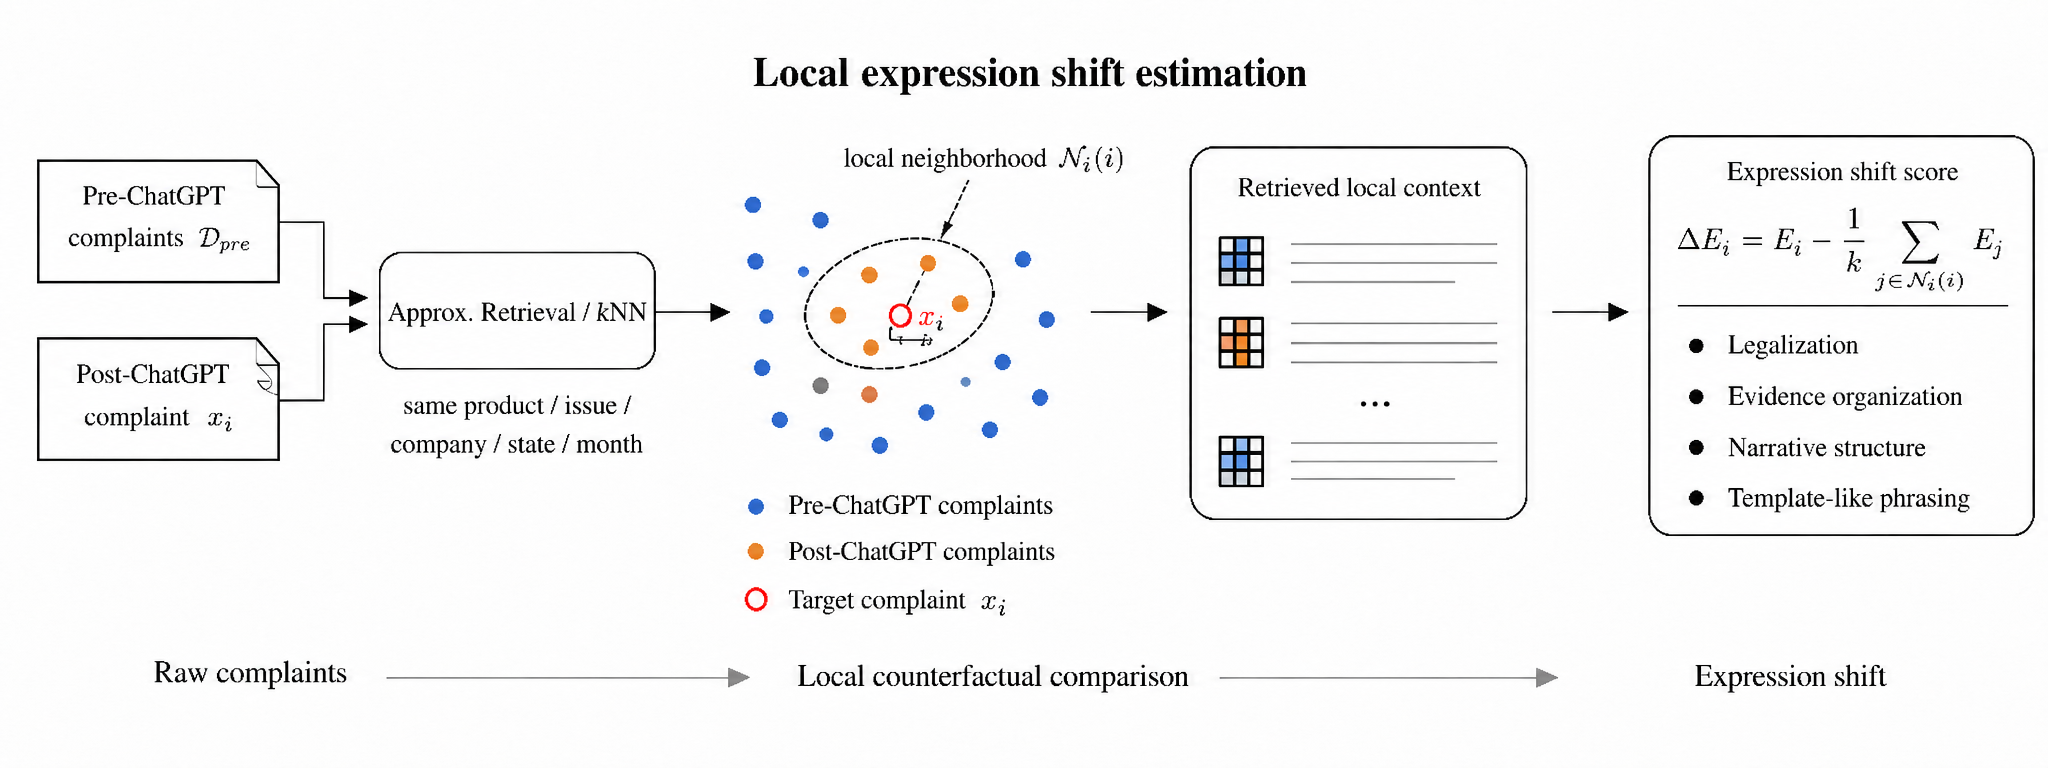
\includegraphics[width=\linewidth]{figures/fig2_local_expression_shift.png}
  \vspace{1em}
  \refstepcounter{figure}
  \label{fig:local-expression-shift}
  \begin{minipage}{0.96\linewidth}
    \raggedright
    \small
    \textbf{Figure~\thefigure.} 局部表达变化估计算法。该图展示了如何从 ChatGPT 前后投诉中构造局部对照集合，并计算目标投诉相对于相似历史投诉的表达变化得分。局部邻域用于控制产品、争议问题、公司、地区和时间等可观测差异。
  \end{minipage}
\end{figure}

\subsection{语义主题与响应预测}

在表达变量之外，本文进一步提取投诉文本的语义表示。具体而言，使用 FinBERT、Sentence-BERT 或 LLM2Vec 将投诉文本 \(T_i\) 编码为向量 \(h_i\)，并使用 BERTopic 或相近的嵌入聚类方法获得主题标签 \(Topic_i\)。文本编码用于保留较高维度的语义信息，主题标签则用于提供可解释的风险类别。最终进入预测模型的特征表示为
\[
z_i=[h_i,X_i,Topic_i,\Delta E_i].
\]
其中 \(X_i\) 包括产品类别、公司、州、提交渠道、年份月份和投诉问题等结构化变量。本文将 Logistic Regression 作为透明基线，将 XGBoost 和 LightGBM 作为主预测模型，并将 TabTransformer 作为表格深度学习对照模型。对每一种响应结果 \(m\in\{timely,monetary,policy\}\)，模型估计
\[
\widehat{Y}_i^{(m)}=f_m(z_i).
\]
由于金钱救济等结果可能存在类别不平衡，模型评估优先报告 PR-AUC，同时补充 ROC-AUC、F1 值和校准曲线。训练和测试采用时间顺序切分，并在训练集内部进行交叉验证，以减少未来信息泄漏。

\begin{figure}[!htbp]
  \centering
  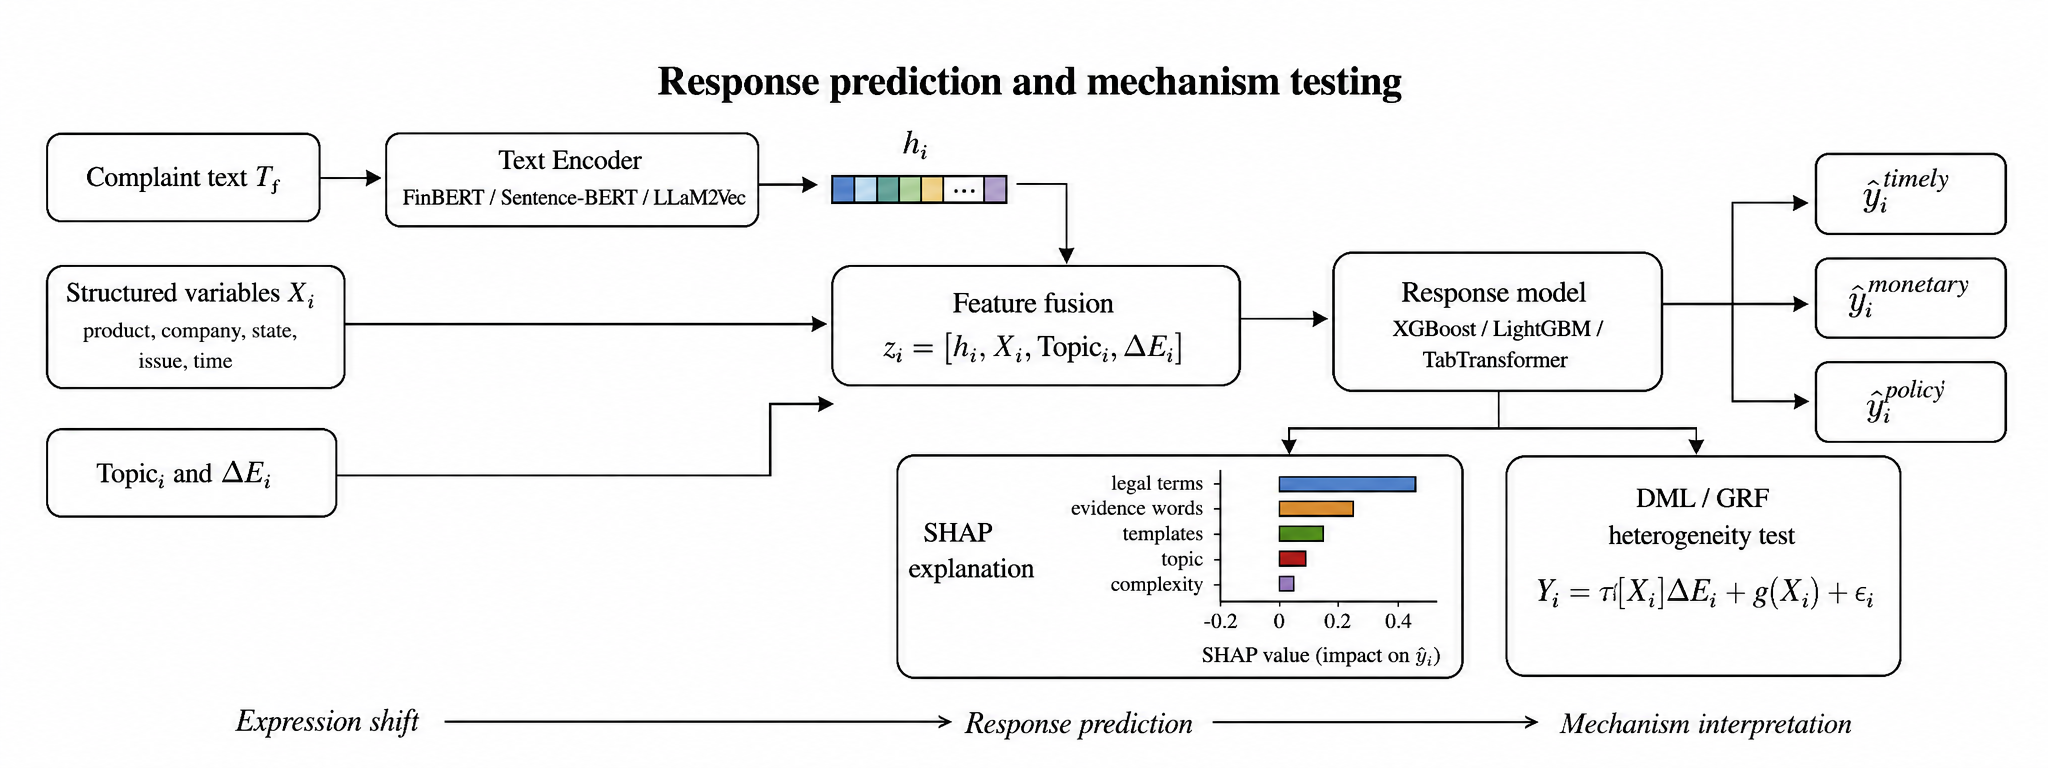
\includegraphics[width=\linewidth]{figures/fig3_response_prediction_mechanism.png}
  \vspace{1em}
  \refstepcounter{figure}
  \label{fig:response-prediction}
  \begin{minipage}{0.96\linewidth}
    \raggedright
    \small
    \textbf{Figure~\thefigure.} 企业响应预测与机制检验框架。投诉文本经编码器得到语义向量，并与结构化变量、主题标签和局部表达变化得分融合，用于预测及时回应、金钱救济和制度性回应。模型解释和异质性检验用于识别哪些表达信号与企业响应结果关系更强。
  \end{minipage}
\end{figure}

\subsection{机制解释与稳健性检验}

预测模型回答的是“哪些变量与企业响应相关”，但并不能直接证明表达变化导致企业回应变化。因此，本文在预测之后加入两类机制检验。第一，使用 SHAP 分解模型输出，观察法律术语、证据词、模板化表达、主题类别和公司变量对预测结果的边际贡献。若法律化或证据化表达在不同模型中持续具有较高贡献，则说明表达组织可能是企业理解投诉的重要信号。第二，将 \(\Delta E_i\) 或高表达变化指示变量作为处理变量，引入双重机器学习或广义随机森林进行异质性分析：
\[
Y_i^{(m)}=\tau_m(X_i)\Delta E_i+g_m(X_i)+\epsilon_i.
\]
其中 \(\tau_m(X_i)\) 表示表达变化在不同产品、公司或地区条件下的异质性关联。本文将该结果解释为机制性证据和稳健性分析，而非完全因果证明。

实验输出将围绕三类图表展开。第一类是表达变化图，用事件研究曲线、分布图和产品类别热力图展示 ChatGPT 前后表达指数的变化。第二类是语义主题图，用 UMAP、主题占比变化和产品--主题热力图展示投诉内容结构。第三类是响应机制图，用模型性能比较、SHAP 重要性和异质性森林图展示文本表达与企业响应之间的关系。这样的图表安排使第三节的算法管线与后续实验结果保持一致：方法图说明如何计算，结果图说明计算之后看到了什么。

\section{实验结果与可视化分析}

本节报告数据清洗后的主要经验结果。本文使用的有效样本共 30,263 条，时间跨度为 2015 年 3 月 20 日至 2026 年 2 月 2 日。由于本地样本中 2024--2026 年记录明显不完整，年度趋势图将其作为不完整样本提示，而不将其解释为真实投诉量下降。以下结果主要用于刻画 ChatGPT 发布前后投诉表达和企业响应的系统差异，并不直接构成因果识别结论。

\subsection{样本结构与企业响应分布}

图 4 展示了样本的基本结构。投诉数量在 2022 年和 2023 年达到本地样本高点，分别为 7,316 条和 7,609 条。以前后分组来看，ChatGPT 发布前样本为 21,788 条，占 72.0\%；发布后样本为 8,475 条，占 28.0\%。从响应结果看，任意救济比例由 21.0\% 上升至 38.4\%，差异为 17.4 个百分点。产品类别高度集中，信用报告类投诉占 64.6\%，债务催收占 16.9\%，信用卡或预付卡占 7.8\%。在企业响应结果中，``closed with explanation'' 占 73.4\%，非金钱救济占 23.0\%，金钱救济仅占 2.9\%。这说明 CFPB 投诉数据的主要经验对象并不是高频金钱赔付，而是企业如何解释、纠正或非金钱性处理消费者争议。

\begin{figure}[H]
  \centering
  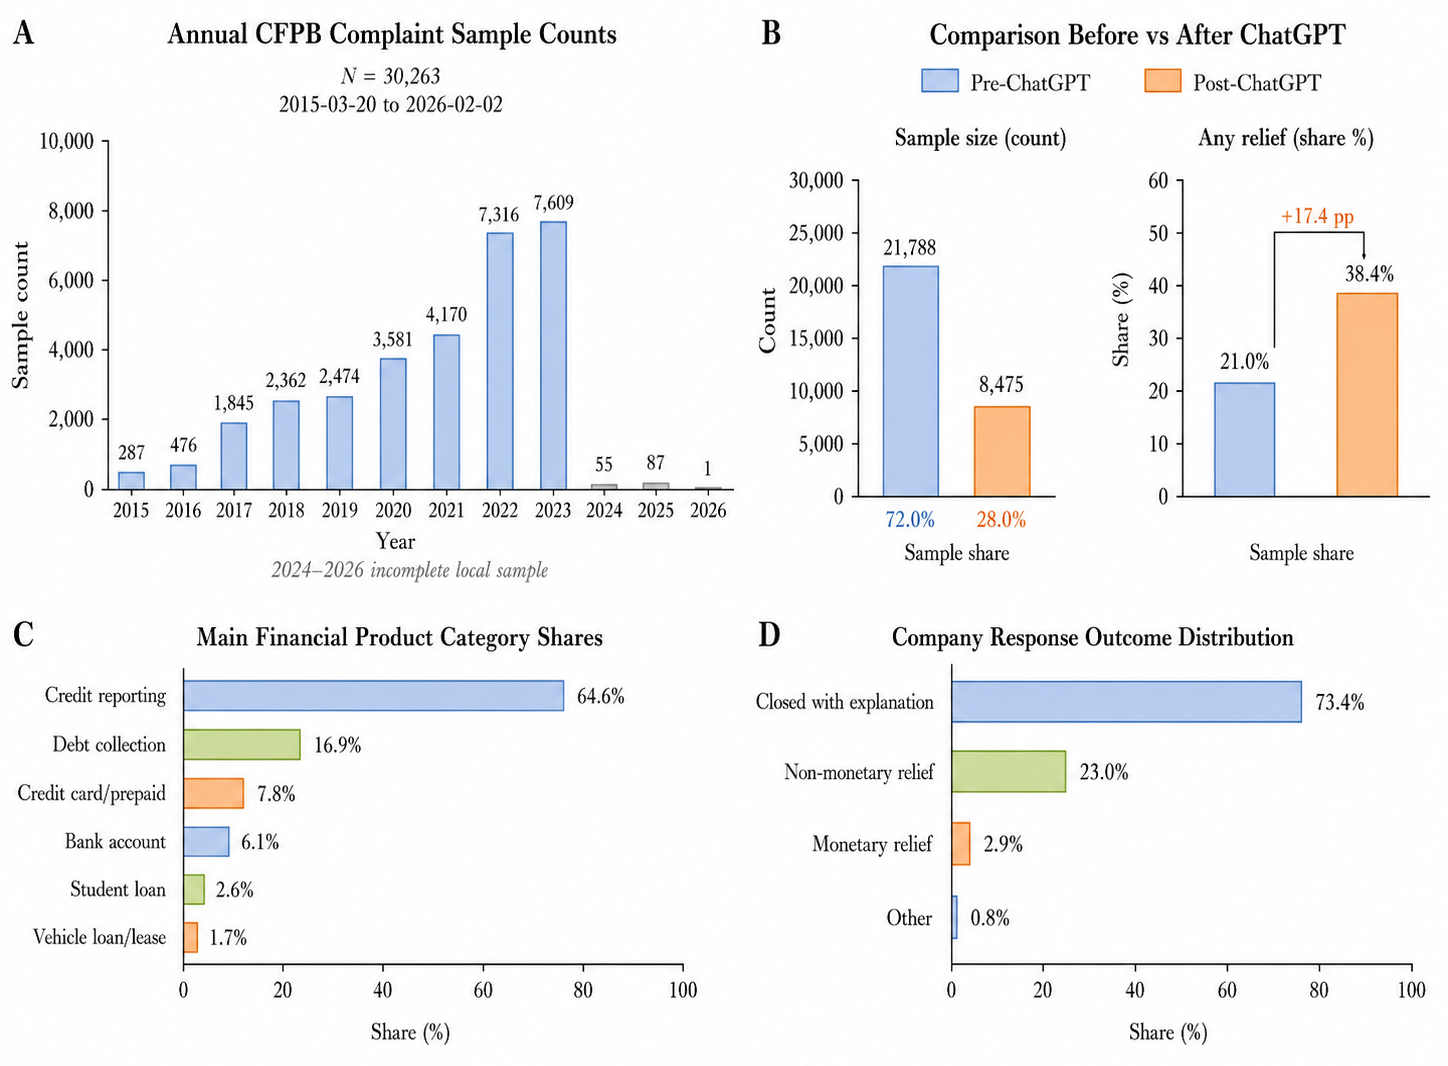
\includegraphics[width=0.86\linewidth]{figures/fig4_sample_overview.png}
  \vspace{1em}
  \refstepcounter{figure}
  \label{fig:sample-overview}
  \begin{minipage}{0.96\linewidth}
    \raggedright
    \small
    \textbf{Figure~\thefigure.} 样本结构、ChatGPT 前后分组与企业响应结果分布。图中报告年度样本量、ChatGPT 发布前后样本占比和任意救济率、主要金融产品类别占比，以及企业响应结果构成。2024--2026 年为本地不完整样本，仅作提示。
  \end{minipage}
\end{figure}

\begin{table}[H]
  \centering
  \footnotesize
  \caption{补充描述统计}
  \label{tab:descriptive-statistics}
  \begin{tabular}{lp{0.68\linewidth}}
    \toprule
    指标 & 数值与说明 \\
    \midrule
    有效样本 & 共 30,263 条；ChatGPT 前 21,788 条，ChatGPT 后 8,475 条 \\
    分类维度 & 产品类别 17 类，争议问题 63 类，公司 1,371 家，州或地区 58 类 \\
    文本长度 & 平均 170.9 词，中位数 113.0 词 \\
    企业回应 & 及时回应率 98.8\%，任意救济率 25.9\% \\
    救济构成 & 金钱救济 2.9\%，非金钱救济 23.0\%，解释性关闭 73.4\% \\
    主要产品 & 信用报告 64.6\%，债务催收 16.9\%，信用卡或预付卡 7.8\% \\
    \bottomrule
  \end{tabular}
\end{table}

\subsection{投诉文本表达的变化}

图 5 进一步比较了 ChatGPT 发布前后的文本表达变量。总体上，投诉文本的平均词数由 169.5 增至 174.4，平均句长由 21.87 增至 23.24，法律术语数由 1.55 增至 3.00，模板化短语数由 0.385 增至 1.040。与此同时，证据词数由 1.19 降至 1.01，词汇多样性由 0.608 降至 0.588。这个组合并不意味着投诉简单变长，而更接近一种表达方式的重组：文本更倾向于使用正式、法律化和模板化语言，但词汇变化空间略有收缩。

产品层面的异质性更加明显。信用报告类投诉的词数增加 23.5，法律术语增加 1.54，模板化短语增加 0.72，任意救济率上升 20.2 个百分点，是表达变化和响应变化最集中的类别。相反，银行账户类投诉平均词数下降 29.5，任意救济率下降 4.6 个百分点。信用卡或预付卡投诉虽然词数减少 47.4，但任意救济率仍上升 5.0 个百分点。这说明 LLM 时代的表达变化并不是所有金融产品中的同向变化，而是与投诉对象、争议类型和既有制度规则密切相关。

\begin{figure}[H]
  \centering
  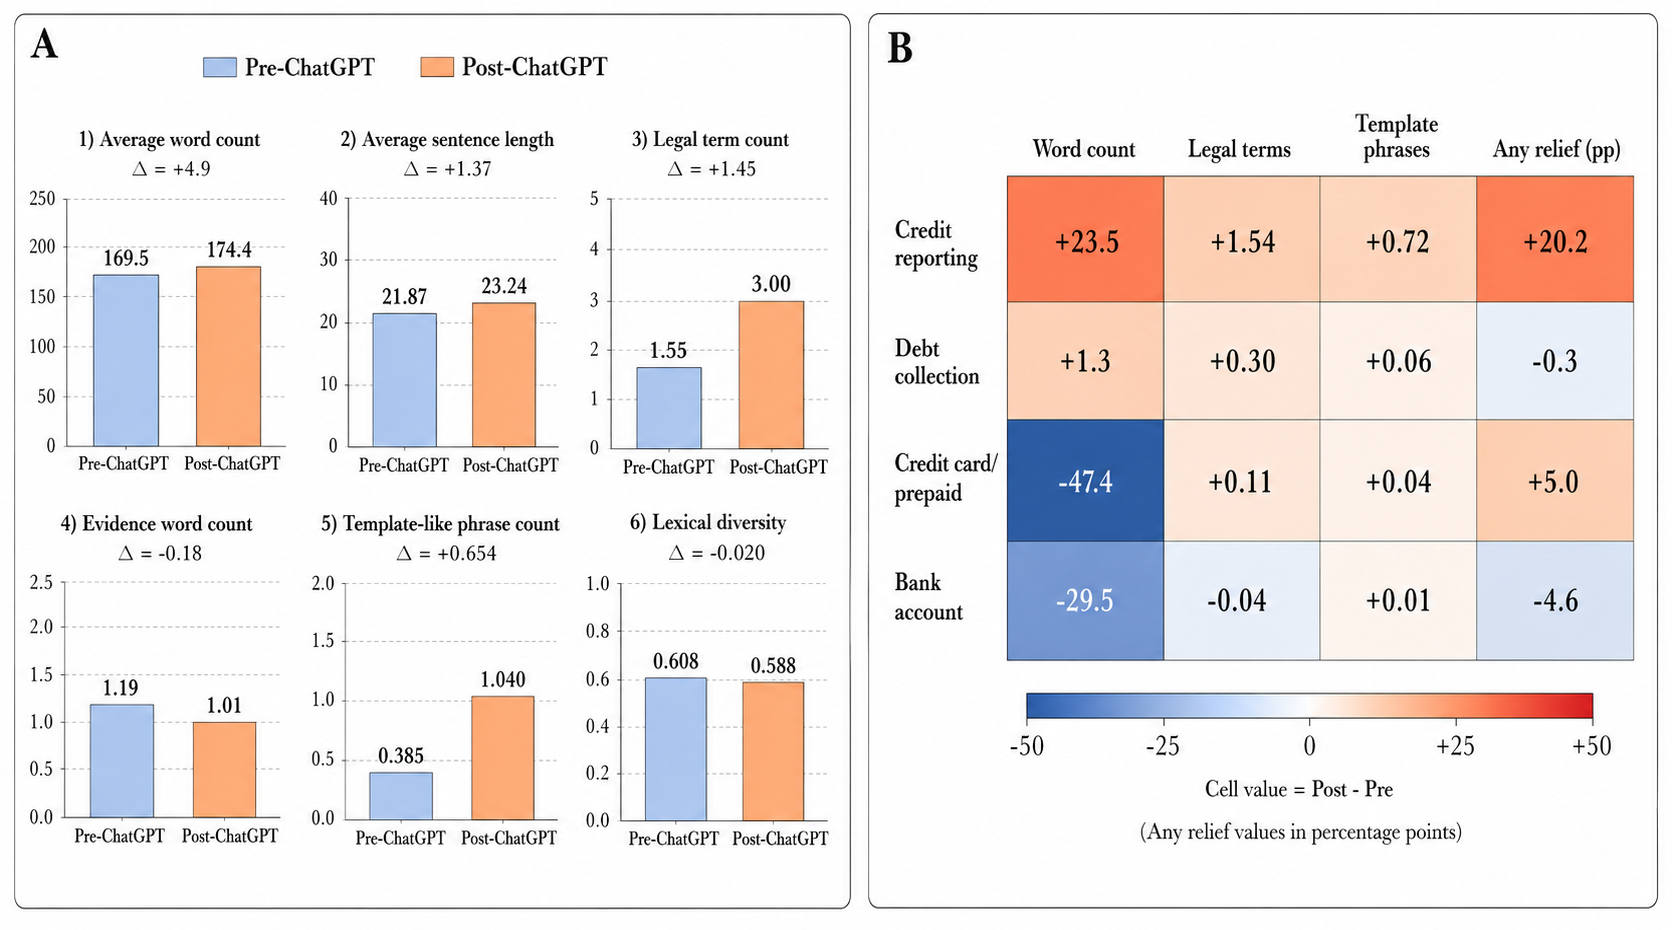
\includegraphics[width=\linewidth]{figures/fig5_expression_shift.png}
  \vspace{1em}
  \refstepcounter{figure}
  \label{fig:expression-shift-results}
  \begin{minipage}{0.96\linewidth}
    \raggedright
    \small
    \textbf{Figure~\thefigure.} ChatGPT 发布前后投诉文本表达变化。面板 A 展示平均词数、平均句长、法律术语数、证据词数、模板化短语数和词汇多样性的前后对比；面板 B 展示主要产品类别中表达指标和任意救济率的 post--pre 差异。
  \end{minipage}
\end{figure}

\subsection{主题结构与响应差异}

图 6 报告了 NMF 主题模型识别出的主要投诉主题及其变化。样本中最大的两个主题是身份盗用与信用报告问题（33.4\%）以及支付、银行、信用卡和贷款争议（33.1\%）；债务验证主题占 17.8\%。ChatGPT 发布后，身份盗用与信用报告主题占比由 30.4\% 上升至 40.8\%，而支付争议主题由 36.6\% 降至 24.0\%，债务验证主题由 20.7\% 降至 10.4\%。与此同时，FCRA 法律模板主题和 reporting agency 主题均有所上升，分别由 4.9\% 增至 6.7\%、由 1.1\% 增至 8.3\%。这与前述法律化、模板化表达增强的结果相互呼应。

不同主题对应的企业响应结果差异也较大。Reporting agency 主题的任意救济率最高，为 44.3\%；FCRA legal template 主题为 37.3\%；consent/perjury 主题为 36.0\%；而 debt validation 主题仅为 15.5\%。这说明投诉主题不仅描述消费者遇到的问题，也可能影响企业对投诉的可处理性和回应策略。尤其是在信用报告和征信机构相关主题中，文本中更清晰的规则引用和权利主张可能更容易被企业转化为纠正或非金钱救济。

\begin{figure}[H]
  \centering
  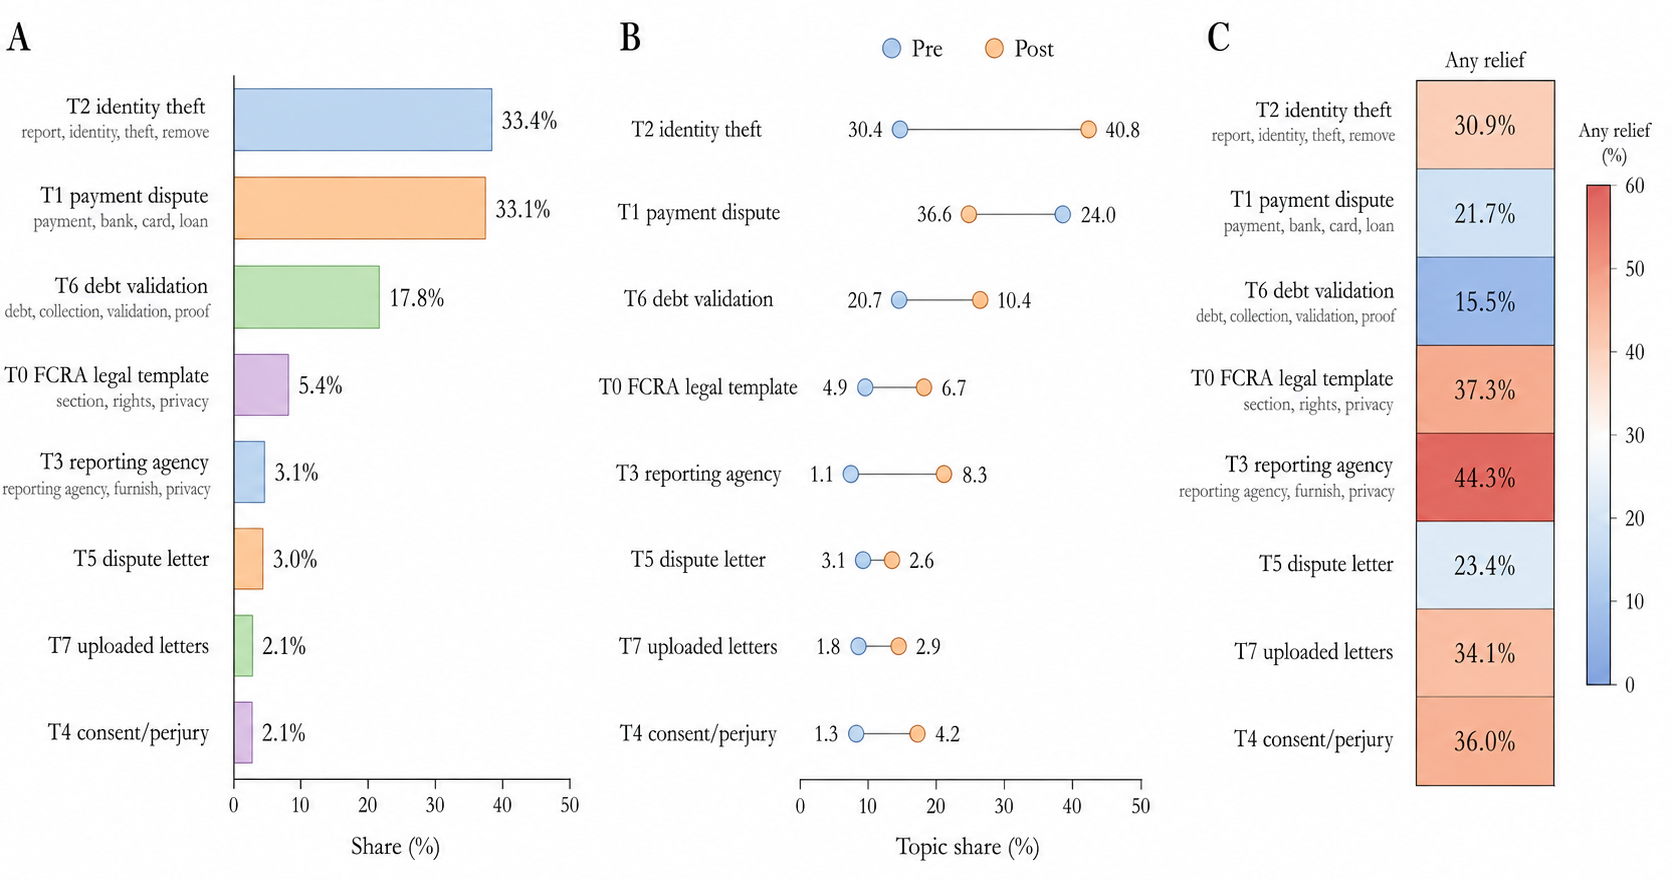
\includegraphics[width=\linewidth]{figures/fig6_topic_structure.png}
  \vspace{1em}
  \refstepcounter{figure}
  \label{fig:topic-results}
  \begin{minipage}{0.96\linewidth}
    \raggedright
    \small
    \textbf{Figure~\thefigure.} 投诉主题结构、ChatGPT 前后主题占比变化与主题响应差异。面板 A 展示主要主题的总体样本占比；面板 B 展示 ChatGPT 发布前后主题占比迁移；面板 C 展示不同主题对应的任意救济比例。
  \end{minipage}
\end{figure}

\subsection{预测性能与解释性特征}

最后，图 7 展示了响应预测模型的主要结果。任意救济预测任务的 ROC-AUC 为 0.710，PR-AUC 为 0.440，F1 值为 0.499，balanced accuracy 为 0.659；及时回应预测任务的 ROC-AUC 为 0.772，PR-AUC 为 0.996，F1 值为 0.960，balanced accuracy 为 0.615。由于及时回应本身的正类比例高达 98.7\%，该任务的 PR-AUC 和 F1 值需要谨慎解释，balanced accuracy 更能反映模型对少数未及时回应样本的识别能力。

特征解释结果显示，任意救济模型中具有较强正向贡献的词项包括 transunion、midland、fraudulent inquiries、impacted data、paypal、fee 和 overdraft 等。这些特征一方面对应公司名称和具体争议场景，另一方面也反映出信用报告、身份盗用和费用争议在救济判断中的重要性。及时回应模型中的正向特征包括 experian、chase、navient、bankruptcy、delete、rights 和 received letter 等，表明机构类型、争议事项和权利表达共同影响回应预测。总体而言，模型结果并不支持一个简单的“文本越像 AI 越容易获得救济”的结论，而是显示文本表达、产品类别、公司和投诉主题共同塑造企业响应。

\begin{figure}[H]
  \centering
  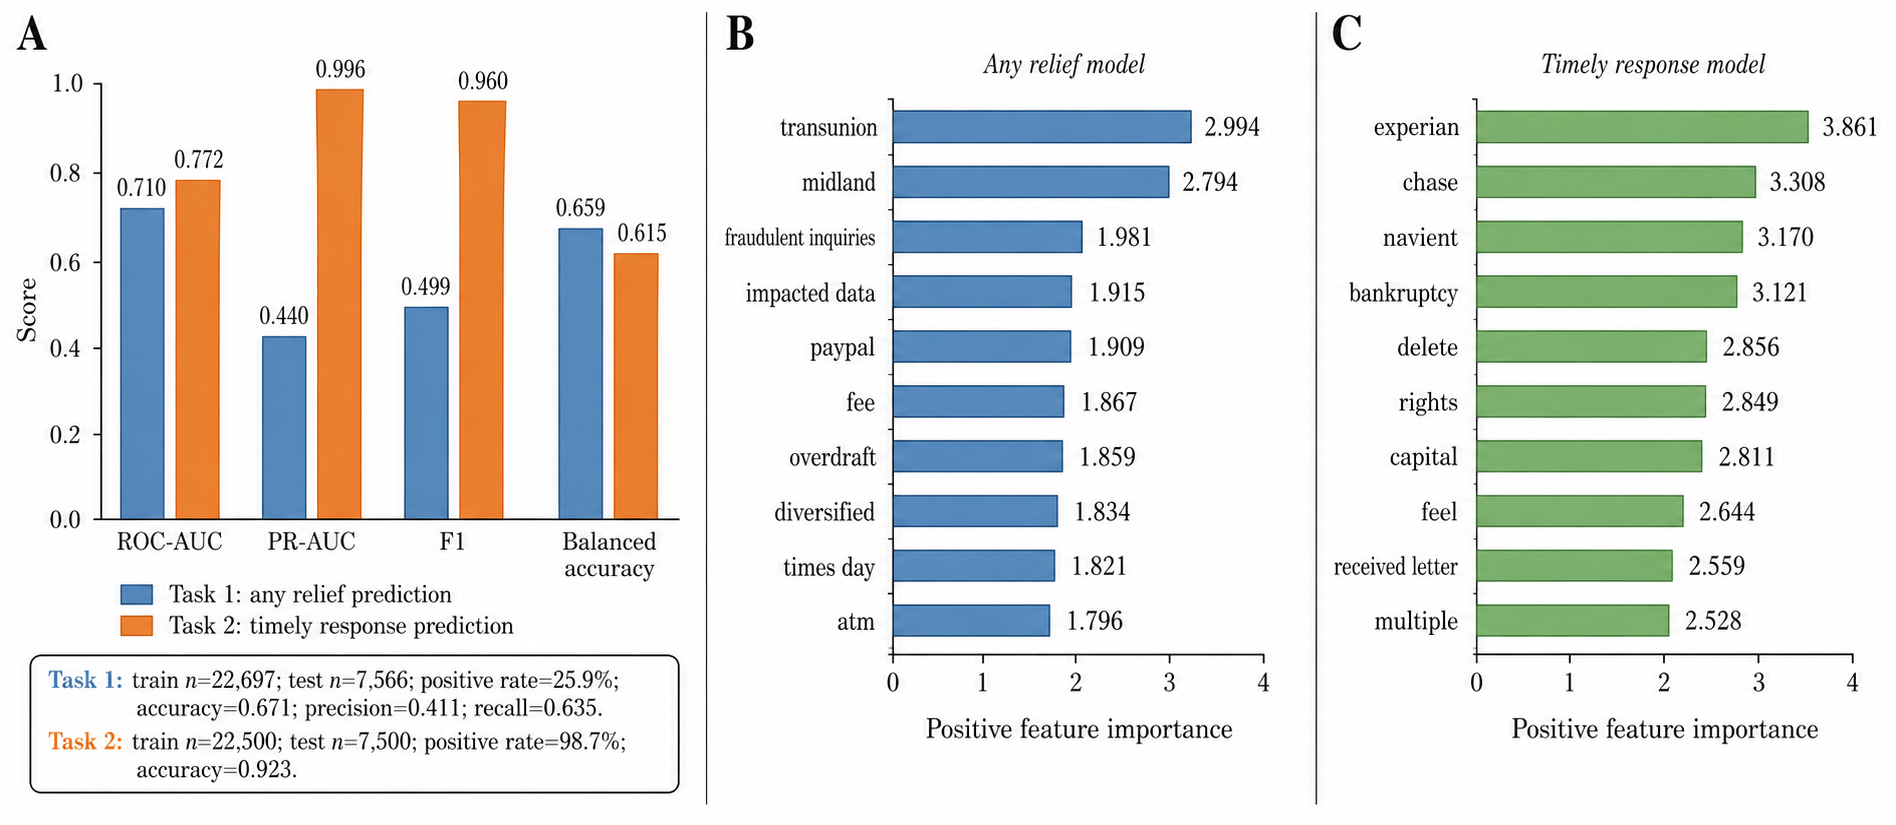
\includegraphics[width=\linewidth]{figures/fig7_model_results.png}
  \vspace{1em}
  \refstepcounter{figure}
  \label{fig:model-results}
  \begin{minipage}{0.96\linewidth}
    \raggedright
    \small
    \textbf{Figure~\thefigure.} 企业响应预测模型性能与正向特征重要性。面板 A 比较任意救济预测和及时回应预测的 ROC-AUC、PR-AUC、F1 与 balanced accuracy；面板 B 和 C 分别展示两个预测任务中的前十个正向特征。
  \end{minipage}
\end{figure}

综合以上结果，后 ChatGPT 时期的 CFPB 投诉文本呈现出更强的法律化和模板化表达，且这种变化主要集中在信用报告、征信机构和身份盗用相关投诉中。企业响应结果也随主题和表达方式发生明显分化：非金钱救济是最主要的救济形式，金钱救济相对少见，预测模型能够捕捉到与公司、争议事项和文本表达相关的响应信号。因而，本文更倾向于将 LLM 理解为一种改变消费者正式表达和信息组织方式的技术条件，而不是简单的投诉自动生成工具。

\section{结论、不足与未来工作}

本文围绕“LLM 能否改变金融投诉的表达方式”这一问题，基于 CFPB 消费者金融投诉数据构建了一个结合文本特征、主题建模和可解释机器学习的分析框架。与既有研究侧重从投诉文本中识别风险主题不同\cite{bastani2019lda,bhattacharya2024shortchanged}，本文进一步将投诉叙事视为一种可能被 LLM 改写的正式表达。经验结果表明，ChatGPT 发布后，投诉文本中的法律术语和模板化短语明显增加，信用报告、身份盗用和征信机构相关投诉是变化最集中的场景；与此同时，任意救济和非金钱救济比例出现上升，预测模型也显示公司、争议主题和表达特征共同影响企业响应。这些结果与近期关于 LLM 辅助写作扩散和 CFPB 投诉中 LLM 采用的研究形成互补\cite{shin2026llmcomplaints,liang2025widespread}，说明生成式 AI 的社会影响不只体现在内容生成本身，也可能体现在弱势消费者如何组织事实、引用规则并提出救济请求。

本文的结论需要在几个边界内理解。第一，本文使用 ChatGPT 发布作为外部时间节点，但这一设计不能完全排除同期监管环境、投诉构成、公司政策和消费者群体变化的影响。因此，本文更适合被解释为文本表达和企业响应之间的系统性关联，而不是严格的因果效应。第二，本文所使用的 AI-like 写作特征只能作为表达变化的代理变量。已有研究表明，机器生成文本检测方法可能受到改写、模型更新和语言背景差异影响\cite{mitchell2023detectgpt,sadasivan2023detection,liang2023detectorsbias}，因此本文没有将单条投诉是否由 AI 生成作为最终判断。第三，本地样本中 2024--2026 年数据不完整，年度趋势不能直接外推到完整 CFPB 数据库。第四，本文主要观察企业是否提供及时回应、金钱救济或非金钱救济，但尚未进一步区分企业内部处理流程、自动化分流机制和消费者后续实际结果。

未来研究可以从三个方向推进。首先，可以将本文框架扩展到完整 CFPB 数据、其他监管投诉平台和多语言消费者文本，检验 LLM 辅助表达是否在不同制度环境下呈现相似模式。其次，可以结合实验设计，让人工参与者或真实投诉文本在有无 LLM 辅助的条件下进行改写，并由人工审阅、检索增强生成和企业响应模拟共同评估文本可读性、证据完整性和救济请求清晰度。此类实验有助于区分“LLM 改变表达方式”和“LLM 使用者本身不同”两种解释。最后，在算法层面，未来工作可进一步结合双重机器学习、广义随机森林、SHAP 和 LIME 等方法，估计表达变化在不同产品、公司和地区中的异质性关联\cite{chernozhukov2018dml,athey2019grf,lundberg2017shap,ribeiro2016lime}。

更广泛地看，LLM 和基础模型的部署带来了效率、可及性与偏误风险并存的制度问题\cite{ouyang2022instructgpt,bommasani2021foundation,bender2021stochastic}。在金融消费者保护场景中，表达能力并不是一个中性的技术变量：它会影响消费者能否把复杂经历转化为企业和监管平台可处理的文本，也会影响机构是否能够准确识别争议的事实、规则和救济请求。因此，后续研究不应只问“AI 是否帮助消费者写得更好”，还应进一步追问这种表达增强是否公平地改善了消费者与机构之间的信息不对称，以及企业自动化响应系统是否会对更模板化、更法律化的文本产生新的选择性偏好。

\bibliographystyle{plain}
\bibliography{references}

\clearpage
\appendix
\setcounter{table}{0}
\renewcommand{\thetable}{A\arabic{table}}
\section{补充实验数据}

本附录报告正文图表中未完全展开的实验数值。附表主要用于提高结果的可复核性，而不引入新的因果解释：附表 A1 给出两个响应预测任务的完整评估指标，附表 A2 展示主要主题的样本规模与响应率，附表 A3 补充主要产品类别的响应结果和文本表达统计。

\begin{table}[H]
  \centering
  \scriptsize
  \caption{响应预测模型的补充评估指标}
  \label{tab:appendix-model-metrics}
  \resizebox{\linewidth}{!}{
  \begin{tabular}{lrrrrrrrrrr}
    \toprule
    预测任务 & 训练集 & 测试集 & 测试正例率 & ROC-AUC & PR-AUC & F1 & Balanced acc. & Accuracy & Precision & Recall \\
    \midrule
    任意救济 & 22,697 & 7,566 & 25.9\% & 0.710 & 0.440 & 0.499 & 0.659 & 0.670 & 0.411 & 0.635 \\
    及时回应 & 22,500 & 7,500 & 98.7\% & 0.771 & 0.995 & 0.960 & 0.615 & 0.923 & 0.991 & 0.931 \\
    \bottomrule
  \end{tabular}}
\end{table}

\begin{table}[H]
  \centering
  \scriptsize
  \caption{主要投诉主题的样本规模、关键词与响应率}
  \label{tab:appendix-topic-response}
  \begin{tabular}{llp{0.27\linewidth}rrrrr}
    \toprule
    主题 & 简要标签 & 代表关键词 & \(n\) & 占比 & 任意救济 & 金钱救济 & 非金钱救济 \\
    \midrule
    T2 & 身份盗用 & report, identity, theft, remove & 10,092 & 33.3\% & 30.9\% & 0.1\% & 30.8\% \\
    T1 & 支付争议 & payment, bank, card, loan & 10,002 & 33.1\% & 21.7\% & 8.5\% & 13.2\% \\
    T6 & 债务验证 & debt, collection, validation, proof & 5,396 & 17.8\% & 15.5\% & 0.2\% & 15.3\% \\
    T0 & FCRA 法律模板 & section, rights, privacy & 1,640 & 5.4\% & 37.3\% & 0.1\% & 37.2\% \\
    T3 & 征信机构 & reporting agency, furnish, privacy & 951 & 3.1\% & 44.3\% & 0.0\% & 44.3\% \\
    T5 & 争议信函 & deleted, letter, response & 902 & 3.0\% & 23.4\% & 0.0\% & 23.4\% \\
    T7 & 上传信件 & uploaded letters, review & 646 & 2.1\% & 34.1\% & 0.0\% & 34.1\% \\
    T4 & 授权与伪证 & consent, perjury, authorization & 634 & 2.1\% & 36.0\% & 0.2\% & 35.8\% \\
    \bottomrule
  \end{tabular}
\end{table}

\begin{table}[H]
  \centering
  \scriptsize
  \caption{主要产品类别的响应结果与文本表达统计}
  \label{tab:appendix-product-response}
  \resizebox{\linewidth}{!}{
  \begin{tabular}{lrrrrrrr}
    \toprule
    产品类别 & \(n\) & 任意救济 & 金钱救济 & 非金钱救济 & 及时回应 & 平均词数 & 法律术语数 \\
    \midrule
    Credit reporting & 19,547 & 30.0\% & 0.2\% & 29.8\% & 99.6\% & 153.4 & 2.62 \\
    Debt collection & 5,115 & 13.2\% & 0.9\% & 12.3\% & 95.5\% & 173.5 & 1.26 \\
    Credit card/prepaid & 2,368 & 31.8\% & 18.9\% & 12.9\% & 99.1\% & 222.7 & 0.34 \\
    Bank account & 1,858 & 22.0\% & 17.0\% & 5.1\% & 98.5\% & 233.5 & 0.19 \\
    Student loan & 799 & 9.8\% & 2.0\% & 7.8\% & 98.0\% & 239.1 & 0.18 \\
    Vehicle loan/lease & 515 & 9.7\% & 3.3\% & 6.4\% & 98.0\% & 230.0 & 0.67 \\
    Mortgage & 38 & 5.3\% & 0.0\% & 5.3\% & 100.0\% & 285.2 & 0.58 \\
    Money transfer & 12 & 16.7\% & 8.3\% & 8.3\% & -- & 190.3 & 0.92 \\
    \bottomrule
  \end{tabular}}
\end{table}

\end{document}
